\documentclass{article}
\usepackage{graphicx}
\usepackage[margin=0.7in]{geometry}
\usepackage[parfill]{parskip}
\usepackage[utf8]{inputenc}
\usepackage{amsmath,amssymb,amsfonts,amsthm}
\usepackage{csquotes}
\MakeOuterQuote{"}

\begin{document}

This post describes a potential attack on certain implementations of plasma cash.

Suppose for concreteness we have the following exit procedure. We reuse the challenge type definitions from https://ethresear.ch/t/plasma-cash-plasma-with-much-less-per-user-data-checking/.

1. Anyone can exit their coin by providing the last two transactions in the coin’s ownership history (ie. the coin they are exiting C and its parent P(C)). This sets a deadline $T$ at some number of blocks into the future (say `T = block.number + 80600`) and initializes a counter $h = 0$ representing the number of unaswered challenges.

2. Challenges can be made before $T$; a type (i) and type (ii) challenge cancels the exit; a type (iii) challenge is written to storage and $h$ is incremented

3. At any time, $h$ can be decremented by providing a response to a type (iii) challenge (which is then deleted)

4. An exit with $h = 0$ can be finalized when `block.number $>$ T`.

Then the following rearrangement attack is possible:

1. Alice signs a transaction to Bob and provides the signature to the operator.

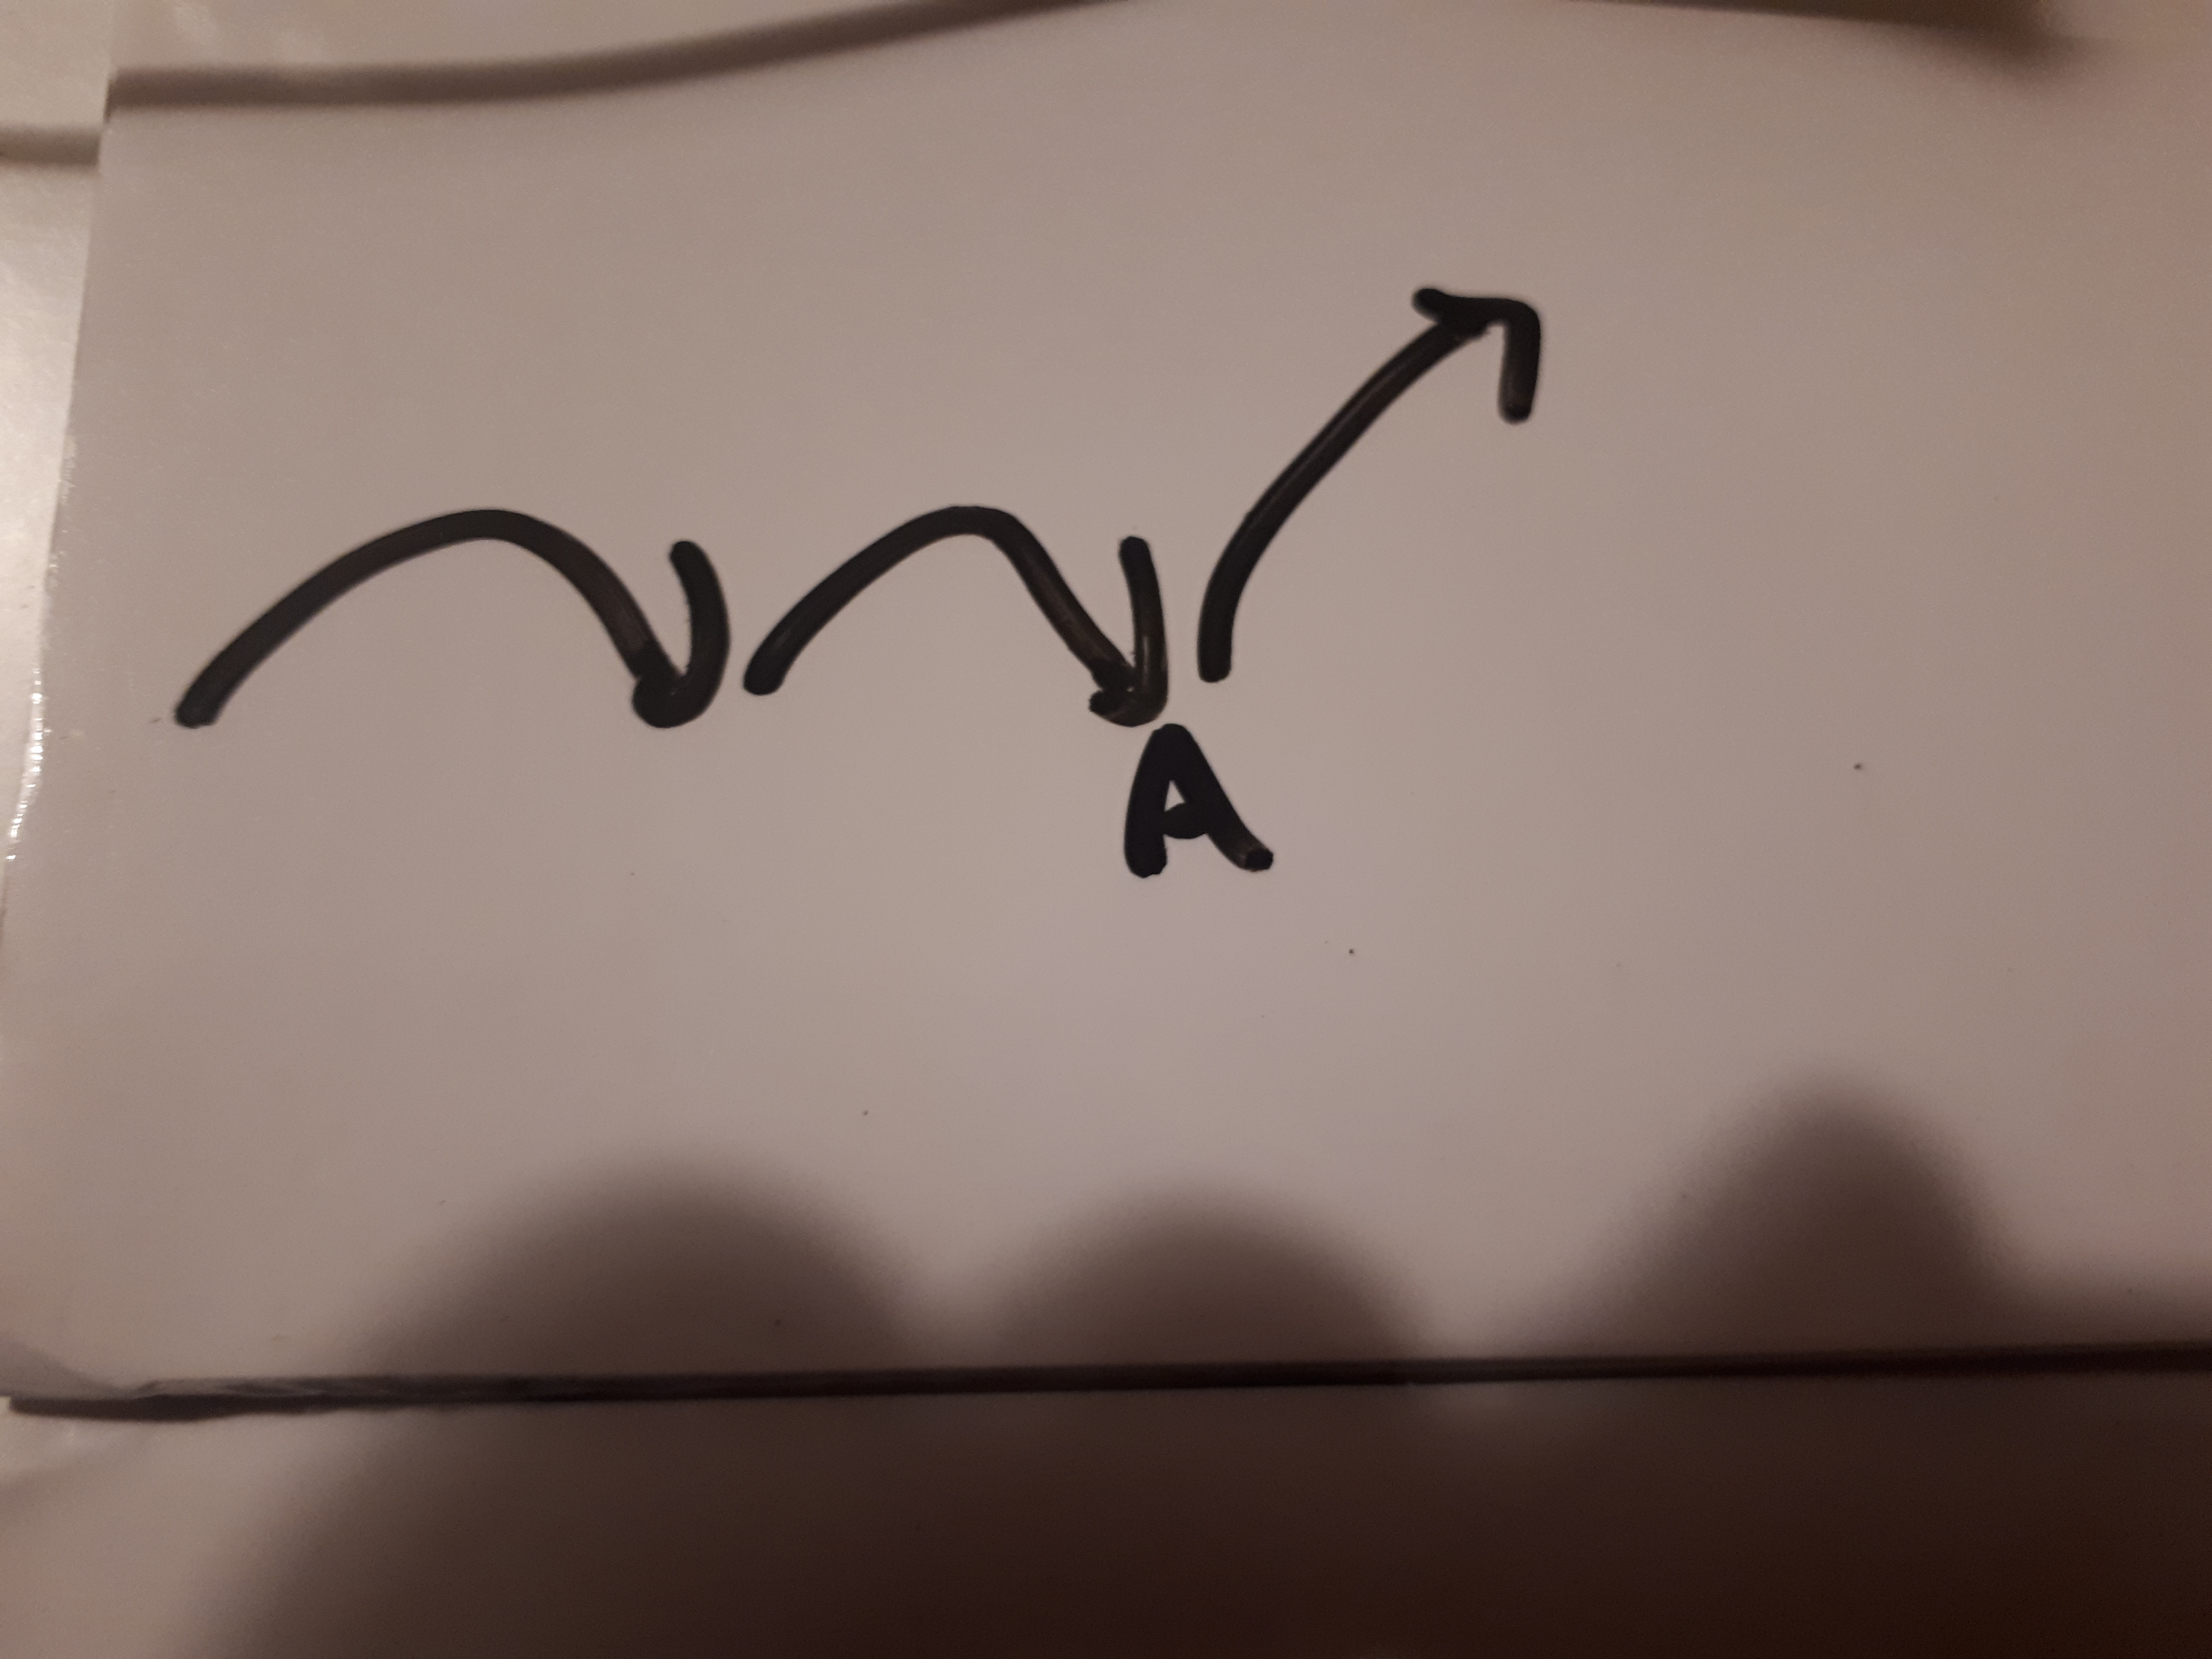
\includegraphics[width=10cm]{A.jpeg}

2. The operator includes a double-spend from E, some spends of that, includes the spend to B among them, and withholds all the blocks

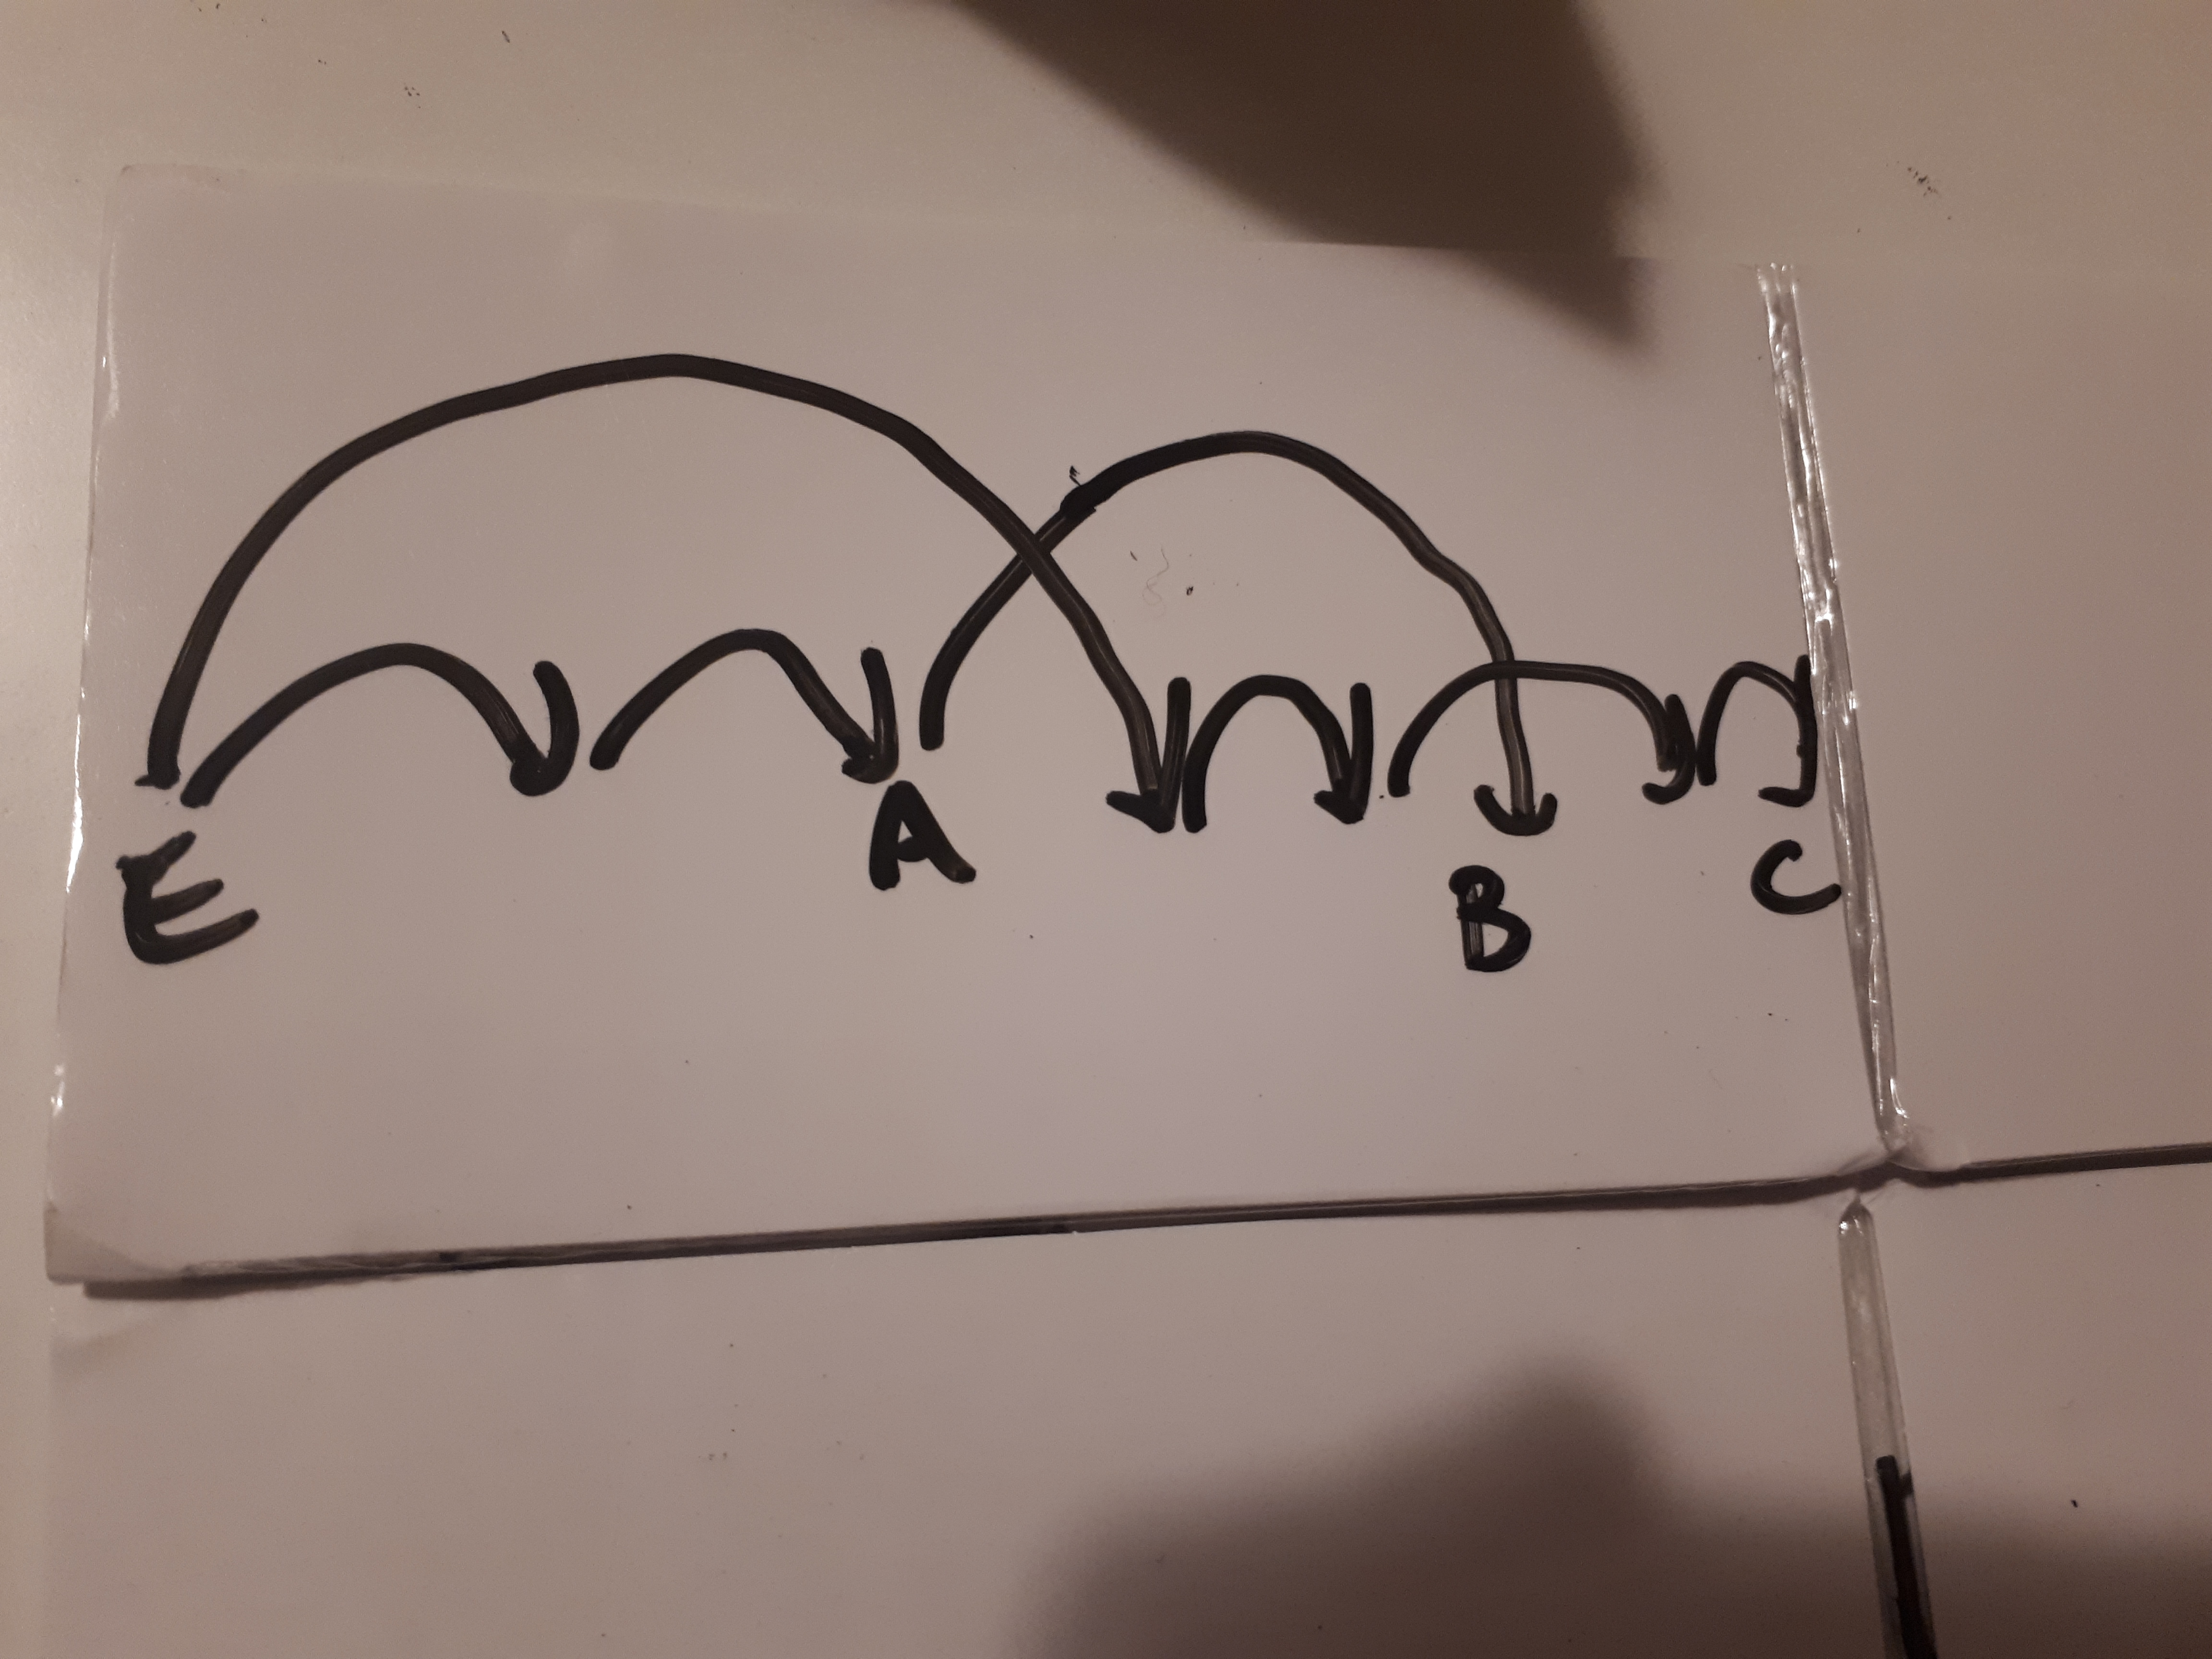
\includegraphics[width=10cm]{B.jpeg}

3. Eve exits coin C
4. The only challenge possible is a type 3 challenge with coin A
5. Eve waits until the block height is greater than T to reveal B, cancelling the challenge
6. It is too late to start a new exit with $B$

Note that similar attacks are possible against many variants of the exit game round structure; if we require that $h$ be set to 0 before $T$ then $B$ can be revealed at block height $T-1$. The general attack is to reveal $B$ "as late as possible". An equivalent statement is that the exit game requires 5 inclusion proofs in the worst case (and not 4 as a naive analysis might conclude) and that the round structure must support this. An example of a round structure not vulnerable to this attack is https://ethresear.ch/t/limbo-exits-and-challenging-fraudulent-exits/.

\end{document}
